\documentclass{amsart}
\usepackage{amsmath,amssymb,amsthm}
\usepackage[T1]{fontenc}
\usepackage{tikz,pgf}
\usetikzlibrary{positioning}
\usetikzlibrary{arrows}
\usetikzlibrary{arrows}
\usetikzlibrary{decorations.pathreplacing}
\usetikzlibrary{calc}

\begin{document}

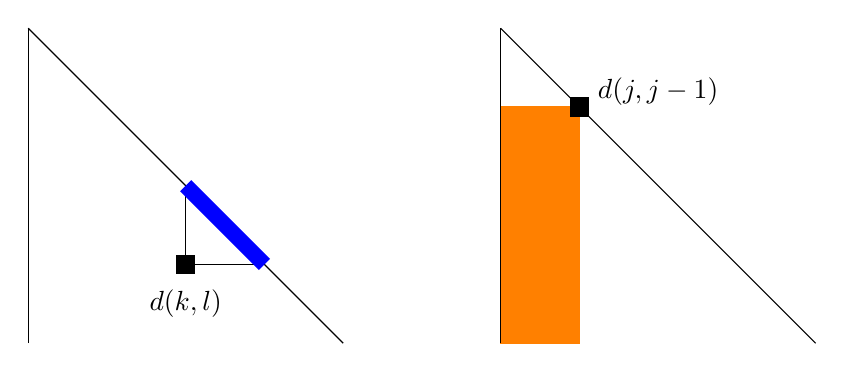
\begin{tikzpicture}

        \draw (0,0) -- (0,4);
        \draw (0,4) -- (4,0);
        \node [fill, draw] at (2,1) {};
        \draw (2,1) -- (2,2);
        \draw (2,1) -- (3,1);
        \node at (2, 0.5) {$d(k,l)$};
        \draw[line width=0.2cm, blue] (2,2) -- (3,1);
        
        \draw[fill=orange, orange] (7,3) rectangle (6,0);

        \draw (6,0) -- (6,4);
        \draw (6,4) -- (10,0);
        \node [fill, draw] at (7,3) {};
        \node at (8, 3.2) {$d(j,j-1)$};

    \end{tikzpicture}

\end{document}